\documentclass[11pt,answers]{exam}

\usepackage{etex}
\usepackage{amssymb,amsmath,multicol} %<-- InWorksheetExam1 i also have fancyhdr,

\usepackage[metapost]{mfpic}
\usepackage[pdftex]{graphicx}

\usepackage{pst-plot}
\usepackage{pgfplots}
\pgfplotsset{compat=1.9}

\usepackage{tikz}
\usepackage{tkz-2d}
\usepackage{tkz-base}
\usetikzlibrary{calc}

\usepackage[inline]{enumitem}
\usepackage{refcount}%<-- non in WorksheetExam1

%\renewcommand{\headrulewidth}{0pt}

\newcommand{\vasymptote}[2][]{
    \draw [densely dashed,#1] ({rel axis cs:0,0} -| {axis cs:#2,0}) -- ({rel axis cs:0,1} -| {axis cs:#2,0});
}

\addpoints
%\printanswers
\noprintanswers

\opengraphsfile{Exam1aaa_Spring_15}

\begin{document}
\extrawidth{-0.3in}
\pagestyle{headandfoot}

\setlength{\hoffset}{-.25in}

\extraheadheight{-.4in}
\runningheadrule
\firstpageheader{\bfseries {MATH1-UC 1171}}{ \bfseries {Exam 1 }}{\bfseries {3/10/2015}} 



\firstpagefooter{\bfseries{}}{}{} 


\runningheader{\bfseries {}}%
              {\bfseries {}}%
              {Page \thepage\ 
							of \numpages 
							}
\runningfooter{} %%&&CHANGED
                {}
                {Points earned: \hbox to 0.5in{\hrulefill}
                 out of  \pointsonpage{\thepage} points}
                 
						

\vspace*{0.7cm}
\hbox to \textwidth { \scshape {Name:} \enspace\hrulefill}
\vspace{0.2in}

\begin{itemize}
	\item This exam contains \numpages\ pages, including this cover page and the blank last page which you can tear out and use as scrap paper. Enter
your name on the top of this page, and put your initials
on the top of every page. Please note that I will not grade anything that you write on the last (blank) page.

%\item Please read the instructions for each individual problem carefully. Try not to overthink a problem and read between the lines! Take your time to solve each problem, and don't rush to finish!
%\item Write legibly and clearly label your answers. If I cannot read your solution to a problem, the problem will receive a score of zero.
\item Calculators may not be used in this exam. You may use your note-card with fomulas/examples. 

\item Please write your name on your note-card and include it in your exam. If you do not have a note-card, please write {\textit {no note-card}} on this page.
\item Turn off all phones and computers, and remove all headphones.

\end{itemize}

For the problems where you are required to show your work, the following rules apply:\\

\begin{minipage}[t]{3.7in}
\vspace{0pt}
\begin{itemize}

\item \textbf{Write in complete sentences}, explaining your calculations, graphs and tables. If you draw a graph, you must label the axes, include tick marks and include units both on the horizontal and vertical axis. If you are asked to explain in practical terms, then your explanation cannot contain math symbols or formulas.
\item \textbf{Use the methods described in this course} as part of your explanations: for example, you cannot use derivatives to find the peaks and valley of a function.

\item \textbf{Organize your work}, neatly and legibly in
the space provided. Work that is disorganized and difficult to read will not receive full credit.  

\item \textbf{A correct answer, unsupported by calculations, explanation,
or algebraic work will receive no credit}; an incorrect answer supported
by  calculations and explanations may receive
partial credit.


\item \textbf{If you need more space}, use the back of the pages; clearly indicate when you have done this.
\end{itemize}

Do not write in the table to the right.
\end{minipage}
\hfill
\begin{minipage}[t]{2.3in}
\vspace{0pt}
%\cellwidth{3em}
\gradetablestretch{2}
\vqword{Pages}
\addpoints % required here by exam.cls, even though questions haven't started yet.	
\combinedgradetable[v][pages]  % Use [pages] to have grading table by page instead of question

\end{minipage}
\newpage

%\bigskip

%\begin{center}
%\gradetable[v][pages]
%\end{center}

%\newpage

\pointpoints{point}{points}

\begin{questions}


\addpoints
%\qformat{Question \thequestion\dotfill
%         {(\pointsofquestion{\arabic{question}} \points)}}

%\bonusqformat{Bonus Question \thequestion\dotfill
%         {(\bonuspointsofquestion{\arabic{question}} \points)}}        
        
%%%%%%%%%%%%%%%%
%No explanations are required for the problems on this page.

%% ONE 1 point  From quiz 
\question  The function $\displaystyle g(x)=|x-3|$ (shown below) is not one-to-one.

\begin{mfpic}[15]{-1}{7}{0}{5}
\arrow \reverse \arrow \polyline{(-0.5,3.5),(3,0),(6.5,3.5)}
\axes
\tlabel[cc](7,-0.5){\scriptsize $x$}
\tlabel[cc](0.5,5){\scriptsize $y$}
\point[3pt]{(3,0),(0,3)}
\xmarks{1,2,3,4,5}
\ymarks{1,2,3,4}
\tcaption{$g(x) = |x-3|$}
\tlpointsep{4pt}
\axislabels {x}{ {\tiny $1$} 1, {\tiny $2$} 2, {\tiny $3$} 3, {\tiny $4$} 4, {\tiny $5$} 5}
\axislabels {y}{{\tiny $1$} 1, {\tiny $2$} 2, {\tiny $3$} 3, {\tiny $4$} 4}
\end{mfpic}
\smallskip

\begin{parts}
\part[1] \label{part:good} Restrict the domain so that the resulting function is one-to-one.

\begin{oneparchoices}
\choice $[2,\infty)$;
\choice $(2,\infty)$;
\choice $[3,\infty)$;
\choice $(-\infty,\infty)$;
\choice $(-\infty,4]$.
\end{oneparchoices}
\part[2] (Explanations are required.) Find the inverse function with the restricted domain you chose in part~\ref{part:good}.
\fillwithdottedlines{1in}

$\displaystyle g^{-1}(x)=$\dotfill
 
\end{parts}



\question 

The domain of the function $\displaystyle f(x)=x^2-4x$ has been restricted to $(-\infty,2]$. 

\begin{parts}
\part[1] Find the range of $f$.

\begin{oneparchoices}
\choice $(-\infty,\infty)$;
\choice $[0,\infty)$;
\choice $[4,\infty)$;
\choice $[-4,\infty)$;
\choice None of these.
\end{oneparchoices}
\part[2] Graph the function $f$ in its restricted domain.

\begin{mfpic}[15]{-6}{6}{-4}{4}
%\arrow \reverse \arrow \polyline{(-4,1), (0,-3), (4,1)}
\axes
\tlabel[cc](6,-0.5){\scriptsize $x$}
\tlabel[cc](0.5,4){\scriptsize $y$}
%\point[3pt]{(0,-3),(3,0),(-3,0)}
\xmarks{-6,-5,-4,-3,-2,-1,1,2,3,4,5}
\ymarks{-4,-3,-2,-1,1,2,3}
\tcaption{$f(x)$}
\tlpointsep{4pt}
\axislabels {x}{{\tiny $-6 \hspace{7pt}$} -6, {\tiny $-5 \hspace{7pt}$} -5, {\tiny $-4 \hspace{7pt}$} -4,  {\tiny $-3 \hspace{7pt}$} -3, {\tiny $-2 \hspace{7pt}$} -2, {\tiny $-1 \hspace{7pt}$} -1, {\tiny $1$} 1, {\tiny $2$} 2, {\tiny $3$} 3, {\tiny $4$} 4, {\tiny $5$} 5}
\axislabels {y}{{\tiny $-4$} -4, {\tiny $-3$} -3, {\tiny $-2$} -2,{\tiny $-1$} -1, {\tiny $1$} 1, {\tiny $2$} 2, {\tiny $3$} 3}
\end{mfpic}

\part[2] (Explanations are required.) Find $\displaystyle f^{-1}(x)$.
\fillwithdottedlines{1.4in}

$\displaystyle f^{-1}(x)=$\dotfill
\end{parts}

\newpage

\question Let $\displaystyle f(x) = \sqrt{36 - x^2}$
 and $\displaystyle g(x) = x^2 - 36$.
 \begin{parts}
 \part[2] (Explanations are required.) Find and simplify $\displaystyle (g\circ f)(x)$.
 \fillwithdottedlines{1in}

$\displaystyle (g\circ f)(x)=$\dotfill

\part[2] (Explanations are required.) Find the domain and write it in interval form.
  \fillwithdottedlines{1in}

Domain:\dotfill
 \end{parts}

\question[1]  Marcello's Pizza charges a base price of \$13 for a large pizza plus \$4 for each topping. Thus, if you order a large pizza with $x$ toppings, the price of your pizza is given by the function  $f(x) = 13 + 4x$. What does $\displaystyle f^{-1}(25)$ represent? Circle the {\underline{one}} best answer.

\begin{choices}
\choice The number of pizzas you can purchase if the toppings cost \$25 dollars.
\choice The number of toppings on a pizza that costs \$25 dollars.    
\choice The number of pizzas you can purchase for \$25.
\choice The cost of a pizza with $3$ toppings.
\choice The cost of just the toppings on a pizza with $3$ toppings.
\end{choices}

\question 

Consider the polynomial: $\displaystyle y=1-9x^8$. Are the following statements true or false?

\begin{parts}
\part[1] If $x\to -\infty$, then $y\to -\infty$
\begin {oneparchoices}
\choice True \choice False
\end{oneparchoices}
\part[1] If $x\to \infty$, then $y\to -\infty$
\begin {oneparchoices}
\choice True \choice False
\end{oneparchoices}
\end{parts}

\bonusquestion[3] A system of two linear equations in two unknowns is graphed below.

\begin{mfpic}[15]{-2}{5}{-2}{5}
\arrow \reverse \arrow \polyline{(-0.5,-2), (3,5)}
\point[3pt]{(2,3)}
\axes
\tlabel[cc](2.5,2.5){\tiny $(2,3)$}
\xmarks{-1,1,2,3,4}
\ymarks{-1,1,2,3,4}
\tlabel(5,-0.5){\scriptsize $x$}
\tlabel(0.5,5){\scriptsize $y$}
%\tcaption{\scriptsize \centerline{$2x-y=1$} \\ \centerline{\boldmath $y=3$}}
\tlpointsep{4pt}
\axislabels {x}{{\tiny $-1 \hspace{7pt}$} -1, {\tiny $1$} 1, {\tiny $2$} 2, {\tiny $3$} 3, {\tiny $4$} 4}
\axislabels {y}{{\tiny $1$} 1, {\tiny $2$} 2, {\tiny $4$} 4}
%\penwd{1.1pt}
\arrow \reverse \arrow \polyline{(-2,3), (5,3)}
\end{mfpic}

Write the equations of the two lines.

$\left\{ \begin{array}{rcr} y & =  & \, \\ y & = & \, \\ \end{array} \right.$ 

\newpage
\question 

The shaded region in the graph shown below represents a feasible region.

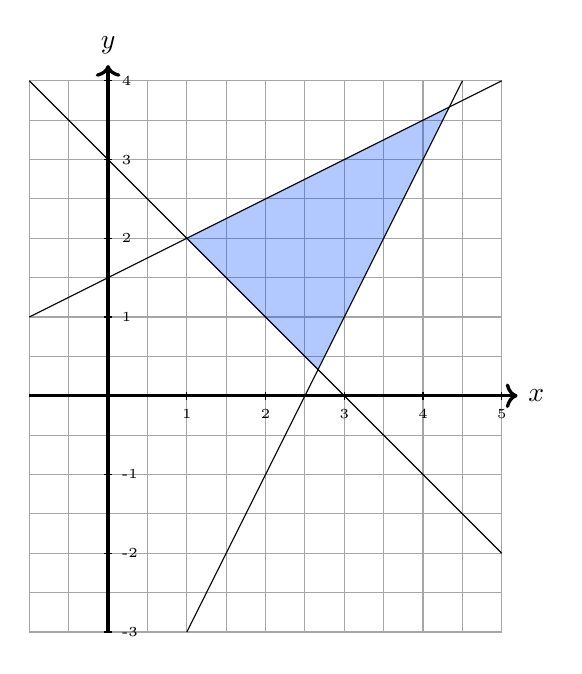
\begin{tikzpicture}

    \draw[gray!70, thin, step=0.5] (-1,-3) grid (5,4);
    \draw[very thick,->] (-1,0) -- (5.2,0) node[right] {$x$};
    \draw[very thick,->] (0,-3) -- (0,4.2) node[above] {$y$};

    \foreach \x in {1,...,5} \draw (\x,0.05) -- (\x,-0.05) node[below] {\tiny\x};
    \foreach \y in {1,...,4} \draw (-0.05,\y) -- (0.05,\y) node[right] {\tiny\y};
    \foreach \y in {-3,...,-1} \draw (-0.05,\y) -- (0.05,\y) node[right] {\tiny\y};

    \fill[blue!70!cyan,opacity=0.3] (8/3,1/3) -- (1,2) -- (13/3,11/3) -- cycle;

    \draw (-1,4) -- node[below,sloped] {} (5,-2);
    \draw (1,-3) -- (3,1) -- node[below left,sloped] {} (4.5,4);
    \draw (-1,1) -- node[above,sloped] {} (5,4);

\end{tikzpicture}

\begin{parts}
\part[1] Is this statement true or false?  One of the inequalities which define the feasible region is $\displaystyle y\leq -x+3$. 

\begin{oneparchoices}
\choice True \choice False
\end{oneparchoices}
\part[1] Is this statement true or false?  One of the inequalities which define the feasible region is $\displaystyle y\geq 0.5x+3$. 

\begin{oneparchoices}
\choice True \choice False
\end{oneparchoices}
\part[1] Is this statement true or false? If the objective function is $\displaystyle M=200-x-y$, then  the maximum of $M$ in the feasible region cannot be at $(3,2)$.

\begin{oneparchoices}
\choice True \choice False
\end{oneparchoices}
\end{parts}

\question[1] Is this statement true or false? The system 

$\begin{cases} 3y-2x=0 \\ 4y+7x=0 \\  \end{cases}$
has exactly one solution.

\begin{oneparchoices}
\choice True \choice False
\end{oneparchoices}

\question

Which of these functions are polynomial functions?

\begin{parts}
\part[1] $\displaystyle y=\frac{4+x^3}{x}$
\begin{oneparchoices}
\choice Polynomial \choice Not polynomial
\end{oneparchoices}
\part[1] $\displaystyle y=\sqrt{x^2+2x+3}$
\begin{oneparchoices}
\choice Polynomial \choice Not polynomial
\end{oneparchoices}
\part[1] $\displaystyle y=|x|$
\begin{oneparchoices}
\choice Polynomial \choice Not polynomial
\end{oneparchoices}
\part[1] $\displaystyle y=x^2+\frac{2}{3}x+\sqrt{3}$
\begin{oneparchoices}
\choice Polynomial \choice Not polynomial
\end{oneparchoices}
\end{parts}
\question[2] (Explanations are required.) The function $L(t)$ represents the number of landlines (per 100 people)  in a certain country $t$ years after 2010. What does the statement $L(3)=39$ mean in practical terms? [Do not write a formula for $L$.]
\fillwithdottedlines{2cm}

\newpage

\question A community bird-watching society makes and sells simple bird feeders to raise money for its conservation activities. The material for each feeder cost \$6, and the society sells an average of 20 per week at a price of \$10 each. The society has been considering raising the price so it conducts a survey and finds that for every dollar increase, it loses 2 sales per week. The profit function is $\displaystyle P(x)=-2 x^2+52 x-240$, where $x$ is the price per feeder.

\begin{parts}
\part[2] (Explanations are required.) What price should the society charge for each feeder to maximize profit?
\fillwithdottedlines{2cm}
Price per feeder:\dotfill

\part[2] (Explanations are required.) What is the maximum weekly profit?
\fillwithdottedlines{2cm}
Maximum profit:\dotfill
\end{parts}

\question The quadratic function $f$ is given by the equation $\displaystyle f(x)=2x^2-4x-6$.

\begin{parts}
\part[3] Explanations are required.) Find the coordinates of the vertex.
\fillwithdottedlines{1.5cm}
Vertex: (\hbox to 0.5in{\dotfill} , \hbox to 0.5in{\dotfill})


\part[2] (Explanations are required.) Find the range of $f$ and write it in interval form.
\fillwithdottedlines{1.5cm}

Range: \hbox to 0.9in{\dotfill} 
\end{parts}

\question[4] Graph a function $f$ with domain $[-1,2]$ and range $[-2,1]$.

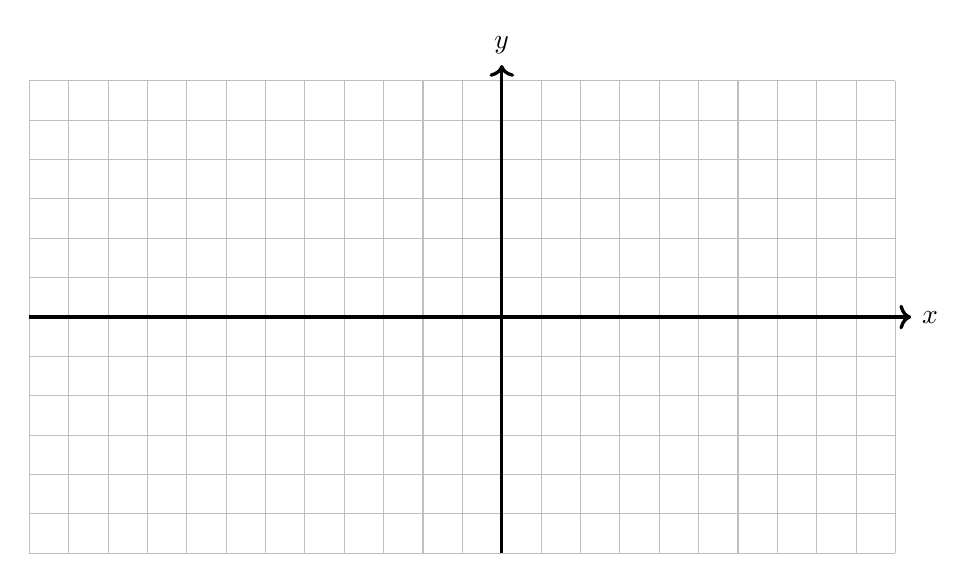
\begin{tikzpicture}


    \draw[gray!50, thin, step=0.5] (-1,-3) grid (10,3);
    \draw[very thick,->] (-1,0) -- (10.2,0) node[right] {$x$};
    \draw[very thick,->] (5,-3) -- (5,3.2) node[above] {$y$};

\end{tikzpicture}

%%%%%%%%\begin{mfpic}[15]{-6}{6}{-4}{4}
%\arrow \reverse \arrow \polyline{(-4,1), (0,-3), (4,1)}
%%%%%%%%\axes
%%%%%%%%\tlabel[cc](6,-0.5){\scriptsize $x$}
%%%%%%%%\tlabel[cc](0.5,4){\scriptsize $y$}
%\point[3pt]{(0,-3),(3,0),(-3,0)}
%%%%%%%%\xmarks{-6,-5,-4,-3,-2,-1,1,2,3,4,5}
%%%%%%%%\ymarks{-4,-3,-2,-1,1,2,3}
%%%%%%%%\tcaption{$f(x)$}
%%%%%%%%\tlpointsep{4pt}
%\axislabels {x}{{\tiny $-6 \hspace{7pt}$} -6, {\tiny $-5 \hspace{7pt}$} -5, {\tiny $-4 \hspace{7pt}$} -4,  {\tiny $-3 \hspace{7pt}$} -3, {\tiny $-2 \hspace{7pt}$} -2, {\tiny $-1 \hspace{7pt}$} -1, {\tiny $1$} 1, {\tiny $2$} 2, {\tiny $3$} 3, {\tiny $4$} 4, {\tiny $5$} 5}
%\axislabels {y}{{\tiny $-4$} -4, {\tiny $-3$} -3, {\tiny $-2$} -2,{\tiny $-1$} -1, {\tiny $1$} 1, {\tiny $2$} 2, {\tiny $3$} 3}
%%%%%%%%\end{mfpic}

\newpage

\question[3] (Explanations are required.) Graph the polynomial function $\displaystyle P(x)=-(x+1)^3+1$ using function transformations of $\displaystyle y=x^3$. Find the exact value of the $y$-intercept and show it on the graph. List all the transformations of $y=x^3$ (in the order that they are performed.)

\fillwithdottedlines{4cm}

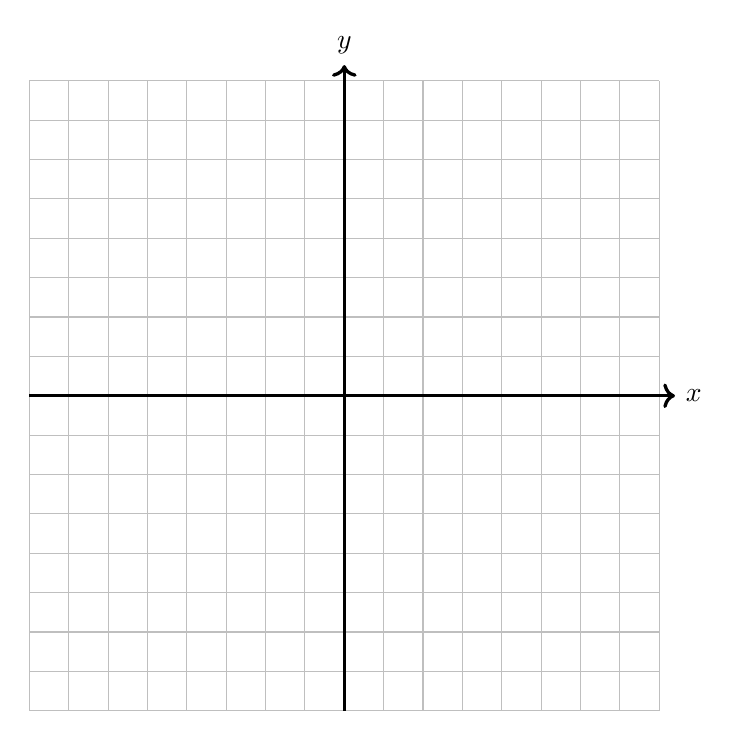
\begin{tikzpicture}

    \draw[gray!50, thin, step=0.5] (-4,-4) grid (4,4);
    \draw[very thick,->] (-4,0) -- (4.2,0) node[right] {$x$};
    \draw[very thick,->] (0,-4) -- (0,4.2) node[above] {$y$};

\end{tikzpicture}

\bonusquestion[1] The domain of $\displaystyle f(x)=x^2+5x+6$ is: 
\begin{oneparchoices}
\choice $(-\infty,-3]\cup [-2,\infty)$
\choice $(-\infty,-3)\cup (-2,\infty)$
\choice $(-\infty,-3)\cup (-3,-2)\cup  (-2,\infty)$
\choice $(-\infty,\infty)$
\choice None of these.
\end{oneparchoices}

\question[1] The domain of $\displaystyle f(x)=\frac{1}{x^2+5x+6}$ is:
 \begin{oneparchoices}
\choice $(-\infty,-3]\cup [-2,\infty)$
\choice $(-\infty,-3)\cup (-2,\infty)$
\choice $(-\infty,-3)\cup (-3,-2)\cup  (-2,\infty)$
\choice $(-\infty,\infty)$
\choice None of these.
\end{oneparchoices}

\question[1] The domain of $\displaystyle f(x)=\sqrt{x^2+5x+6}$ is:
 \begin{oneparchoices}
\choice $(-\infty,-3]\cup [-2,\infty)$
\choice $(-\infty,-3)\cup (-2,\infty)$
\choice $(-\infty,-3)\cup (-3,-2)\cup  (-2,\infty)$
\choice $(-\infty,\infty)$
\choice None of these.
\end{oneparchoices}

\question[1] The domain of $\displaystyle f(x)=\frac{1}{\sqrt{x^2+5x+6}}$ is:
 \begin{oneparchoices}
\choice $(-\infty,-3]\cup [-2,\infty)$
\choice $(-\infty,-3)\cup (-2,\infty)$
\choice $(-\infty,-3)\cup (-3,-2)\cup  (-2,\infty)$
\choice $(-\infty,\infty)$
\choice None of these.
\end{oneparchoices}
\newpage

\question The goal of this problem is to graph the polynomial $\displaystyle P(x)=(x-1)^2(x+1)^3(x-2)$.
\begin{parts}
\part[1] What is the degree of $P$? \hbox to 0.9in{\dotfill}
\part[1] What is the leading coefficient of $P$? \hbox to 0.9in{\dotfill}
\part[1] How many $x$-intercept does the graph of $P$ have? \hbox to 0.9in{\dotfill}
\part[1] What is the $y$-intercept? \hbox to 0.9in{\dotfill}
\part[5] (Explanations are required.) Graph $P$. 
\fillwithdottedlines{3cm}

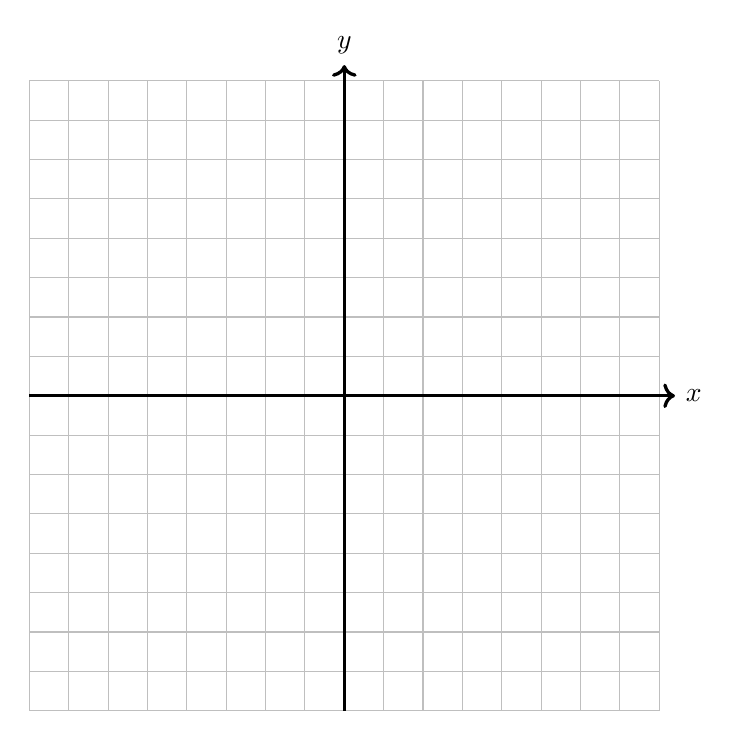
\begin{tikzpicture}

    \draw[gray!50, thin, step=0.5] (-4,-4) grid (4,4);
    \draw[very thick,->] (-4,0) -- (4.2,0) node[right] {$x$};
    \draw[very thick,->] (0,-4) -- (0,4.2) node[above] {$y$};

\end{tikzpicture}

\end{parts}

\question[1] Write a formula for the function $f(x)$ obtained from $\displaystyle y=\sqrt{x}$ by applying the following transformations (in the given order): 
\begin{enumerate*}[series=MyList, before=\hspace{-0.6ex}] 
\item[(a)] reflection around the $y$ axis; \item[(b)] horizontal shift by 3 units to the left.
\end{enumerate*}

$f(x) =$ \hbox to 0.9in{\dotfill} 

\question[1] Write a formula for the function $g(x)$ obtained from $\displaystyle y=\sqrt{x}$ by applying the following transformations (in the given order): 
\begin{enumerate*}[series=MyList, before=\hspace{-0.6ex}] 
\item[(a)] horizontal shift by 3 units to the right;
\item[(b)] reflection around the $y$ axis.
\end{enumerate*}

$g(x) =$ \hbox to 0.9in{\dotfill} 

\bonusquestion[1] Assume that $f$ is a one-to-one function, and that $f(3)=11$. Then $\displaystyle f^{-1}(11)=$\hbox to 0.6in{\dotfill} 

\end{questions}
\newpage
\thispagestyle{empty}


\setlength\fboxrule{2pt}\setlength\fboxsep{2mm}
\fbox{This page is intentionally left blank.} You may use it as scrap paper for your calculations.
\end{document}                 